\documentclass[10pt,twocolumn,letterpaper]{article}

\usepackage[utf8]{inputenc}
\usepackage[margin=0.75in]{geometry}
\usepackage{amsmath,amssymb,amsfonts}
\usepackage{booktabs}
\usepackage{tikz}
\usepackage{hyperref}
\usepackage{microtype}
\usepackage{cite}

\hypersetup{
    colorlinks=true,
    linkcolor=blue!70!black,
    citecolor=blue!70!black,
    urlcolor=blue!70!black,
    pdfauthor={Shriram Baskar},
    pdftitle={Post-Generation Tool Governance for Autonomous AI Agents: A Deterministic Reference-Monitor Architecture and Empirical Evaluation},
    pdfkeywords={Large Language Model Security, Autonomous AI Agents, Indirect Prompt Injection, Execution Governance, Reference Monitor, Access Control}
}

\title{\textbf{\Large Post-Generation Tool Governance for Autonomous AI Agents:\\A Deterministic Reference-Monitor Architecture and Empirical Evaluation}}

\author{\textbf{Shriram Baskar}\\ \small Independent Researcher\\ \small \texttt{https://github.com/Shriram28Baskar/PromptAegis\_RI}}

\date{}

\begin{document}

\maketitle

\begin{abstract}
\textbf{Autonomous language model (LLM) agents interacting with external digital environments inherit significant security risks from indirect prompt injection and context poisoning. While prior research predominantly investigates pre-generation alignment and probabilistic token filtering, these techniques cannot enforce deterministic execution invariants once an attacker manipulates the model's internal reasoning context.}

\textbf{This paper investigates whether deterministic, post-generation execution governance can constrain the security consequences of compromised tool calls while preserving legitimate operational utility and maintaining measurable execution latency. We present \textbf{PromptAegis}, an application-level reference monitor positioned strictly between an agent's structured action proposal and the concrete tool execution dispatcher. \textbf{PromptAegis} mediates routed tool invocations through a sequential five-stage pipeline: volumetric fixed tumbling-window rate limiting, deterministic role-based access control (RBAC), argument-level policy validation incorporating keyword-agnostic parameter canonicalization, risk scoring with approval gating, and structured audit logging.}

\textbf{We evaluate \textbf{PromptAegis} across a primary synthetic benchmark of $N=500$ attack scenarios and $N=100$ benign operational commands. To eliminate confounding between semantic policy inspection and volumetric rate saturation, we implement a mechanism-isolation ablation protocol across six configurations ($3{,}000$ attack evaluations and $3{,}600$ total scenario decisions). Under isolated semantic evaluation with rate limiting inactive, \textbf{PromptAegis} reduces the Attack Success Rate (ASR) from $100.0\%$ ($500/500$) in the unprotected baseline to $40.0\%$ ($200/500$) under RBAC alone, $33.0\%$ ($165/500$) under policy inspection alone, and $30.0\%$ ($150/500$) under combined normalized inspection (McNemar Edwards $\chi^2 = 348.0029, p = 1.15 \times 10^{-77}$). In a calibrated gateway configuration (incorporating refined argument schemas and tool-scoped parameter fallback rules), residual ASR is reduced to $20.4\%$ ($102/500$) on the evaluated benchmark while maintaining a $100.0\%$ ($100/100$) Legitimate Task Completion Rate (LTCR) and $0.0\%$ ($0/100$) False Positive Rate (FPR). The median paired per-scenario latency overhead is $+11.27\text{ ms}$ under normalized traffic and $+13.38\text{ ms}$ under burst traffic.}

\textbf{Adversarial stress testing across 500 mutation instances drawn from a clustered perturbation design ($5$ classes $\times$ $100$ base templates; $2{,}000$ execution evaluations) exposes critical non-monotonic trade-offs: while structural Base64 canonicalization increases isolated evasion block rates from $0.0\%$ ($0/100$) to $50.0\%$ ($50/100$), overall isolated block rate decreases from $40.0\%$ ($200/500$) to $36.4\%$ ($182/500$) because aggressive comment stripping alters string character offsets for secondary regex rules. In compound burst testing, the standard pipeline blocks $75.2\%$ ($376/500$, $24.8\%$ ASR); however, mechanism attribution confirms that $95.74\%$ ($360/376$) of these blocks are driven by rate-limiter saturation rather than parameter inspection. In an exploratory closed-loop pilot ($N=20$) with a live commercial LLM (\texttt{gpt-oss-120b}), \textbf{PromptAegis} intercepted $75.0\%$ ($3/4$) of rogue tool calls emitted following successful prompt injections, limiting unintercepted hostile tool execution to $10.0\%$ ($1/10$).}

\textbf{Our findings indicate that deterministic post-generation governance provides measurable execution mitigation against unauthorized actions, but its protection remains strictly bounded by syntactic policy expressiveness, cannot prevent parameter smuggling within authorized semantic spaces, and does not alter the underlying vulnerability of the model's reasoning.}
\end{abstract}

\vspace{0.5em}
\noindent\textbf{Keywords}---Large Language Model Security, Autonomous AI Agents, Indirect Prompt Injection, Execution Governance, Reference Monitor, Access Control, Parameter Canonicalization.

\section{Introduction}
The integration of Large Language Models (LLMs) into autonomous agentic workflows---such as ReAct~\cite{react}, Toolformer~\cite{toolformer}, and AutoGen~\cite{autogen}---enables generative models to issue executable actions directly against shell environments, databases, and external APIs. This paradigm shift introduces a fundamental challenge in computer systems security: whereas classical security engineering dictates that untrusted input must never determine control flow or execution privileges~\cite{saltzer}, autonomous agents ingest untrusted external context (e.g., retrieved web text, email content, ticketing data) into the prompt context that directs execution planning. Consequently, adversaries can stage \emph{indirect prompt injection} attacks~\cite{greshake}, manipulating the model's internal reasoning into emitting unauthorized, high-privilege, or destructive tool invocations.

Existing defensive strategies focus primarily on \textbf{pre-generation alignment} (e.g., RLHF~\cite{ouyang}) and \textbf{system prompt instructions}, though empirical evaluations demonstrate that natural language instructions fail to reliably prevent prompt injection~\cite{perez}, alongside \textbf{probabilistic token guardrails} (e.g., Llama Guard~\cite{llamaguard}, NeMo Guardrails~\cite{nemoguardrails}). While these techniques raise the cost of basic jailbreaks, they treat security as a statistical property of natural language tokens. Because generative models operate over unsegmented natural language, probabilistic filtering cannot guarantee deterministic execution invariants against out-of-distribution adversarial prompts~\cite{zou}.

This paper investigates an alternative, complementary principle: \textbf{separating reasoning security from execution governance}. An autonomous agent's reasoning engine may be manipulated by adversarial text, but catastrophic outcomes can be prevented if the concrete tool invocations emitted by the model are mediated by an external, application-level \emph{reference monitor}~\cite{anderson,schneider}. Rather than attempting to force the LLM into a provably safe cognitive state, security architectures can treat the model as an untrusted computation engine operating within an adversary's potential sphere of influence.

We design, implement, and evaluate \textbf{PromptAegis}, an application-level, deterministic post-generation tool governance gateway. Positioned strictly between the LLM output parser and the concrete tool execution dispatcher, PromptAegis mediates every proposed function call through a multi-stage deterministic pipeline: 60-second fixed tumbling-window rate limiting, role-based access control (RBAC), argument-level policy inspection incorporating keyword-agnostic parameter canonicalization, risk scoring with approval gating, and audit telemetry.

\subsection{Research Questions}
\begin{itemize}
    \item \textbf{RQ1 (Semantic Efficacy)}: To what extent can deterministic RBAC and argument-level regex policies reduce the Attack Success Rate (ASR) of compromised tool calls in the absence of rate-limiting confounding?
    \item \textbf{RQ2 (Utility Preservation \& False Positives)}: What Legitimate Task Completion Rate (LTCR) and False Positive Rate (FPR) are observed on the benign operational corpus when post-generation policy inspection is applied?
    \item \textbf{RQ3 (Latency Overhead)}: What execution latency overhead does post-generation mediation introduce relative to unmediated tool dispatch?
    \item \textbf{RQ4 (Adversarial Evasion \& Trade-offs)}: How do parameter canonicalization rules perform against obfuscated payloads, and does normalization introduce negative performance trade-offs?
    \item \textbf{RQ5 (Dynamic Closed-Loop Feasibility)}: In an end-to-end agent loop with a live LLM, what proportion of prompt-injection-induced tool calls are intercepted post-generation?
\end{itemize}

\section{Problem Formulation}
Let an autonomous agent $\mathcal{A}$ operate over discrete interaction steps $t \in \{1, \dots, T\}$. At step $t$, the agent receives an environment observation $o_t \in \mathcal{O}$ and interaction history $h_t = (u, o_1, a_1, \dots, o_{t-1}, a_{t-1})$, where $u \in \mathcal{U}$ is the primary user task instruction. Observation $o_t$ may contain untrusted data from external sources. The agent's autoregressive policy $\mathcal{M}_\theta$ emits a token sequence parsed into a structured action proposal:
\begin{equation}
a_t = (r, \tau, \theta_\tau)
\end{equation}
where $r \in \mathcal{R}$ is the active agent role, $\tau \in \mathcal{T}$ is the target tool identifier, and $\theta_\tau \in \Theta_\tau$ is the dictionary of structured arguments.

In an unmitigated architecture, tool dispatch is direct:
\begin{equation}
\mathcal{E}_{t+1} \leftarrow \text{Exec}(\tau, \theta_\tau)
\end{equation}

When an adversary embeds an injection payload $\delta_{\text{adv}}$ within $o_t$, the conditional probability of emitting a malicious tool call $a_t \in \mathcal{A}_{\text{malicious}}$ increases. PromptAegis introduces a deterministic reference monitor function $\mathcal{G}: \mathcal{A} \times \mathcal{S}_{\text{state}} \to \{ \text{ALLOW}, \text{BLOCK}, \text{REQUIRE\_APPROVAL} \}$ such that:
\begin{equation}
\mathcal{G}(a_t) = \begin{cases} 
\text{ALLOW} \implies \text{Exec}(\tau, \theta_\tau) \\ 
\text{BLOCK} \implies \text{Error}(\text{``Policy Violation''}, \epsilon_\tau) \\ 
\text{REQUIRE\_APPROVAL} \implies \text{Halt}(\text{``Confirmation Required''}, \epsilon_\tau) 
\end{cases}
\end{equation}
The operational objective is to minimize ASR ($\text{ASR} \to 0$) while maintaining utility ($\text{LTCR} = 1.0, \text{FPR} = 0.0$) under bounded execution latency.

\section{Threat Model}

\subsection{Attacker Profile \& In-Scope Vectors}
The adversary is an external entity capable of manipulating untrusted text consumed by the agent. The adversary cannot modify model weights, system prompts, gateway source code, or the underlying host OS. We consider five primary operational attack categories ($N=100$ scenarios each):
\begin{itemize}
    \item \textbf{T1: Unauthorized Tool Execution}: Coercing an agent into invoking tools outside its operational mandate (e.g., a support agent calling \texttt{execute\_shell\_command}).
    \item \textbf{T2: Privilege Escalation}: Forcing an agent to execute administrative functions (e.g., \texttt{update\_customer\_role}).
    \item \textbf{T3: Prompt-Driven Restricted Tool Execution}: Inducing high-risk destructive actions under an authorized tool (e.g., calling \texttt{file\_writer} to overwrite \texttt{/etc/hosts}).
    \item \textbf{T4: Parameter Manipulation}: Injecting SQL syntax (\texttt{' OR '1'='1}), shell chaining operators (\texttt{\&\&}, \texttt{|}), or directory traversal paths (\texttt{../../}) into permitted arguments.
    \item \textbf{T5: Excessive Invocations / Volumetric DoS}: Forcing automated recursive loops to exhaust API quotas or scrape data.
\end{itemize}

Separately, an \textbf{Adversarial Perturbation Suite} ($N=500$) evaluates evasion transformations: Base64 encoding, URL percent-encoding, SQL comment fragmentation, case alternation, and stacked SQL logic.

\subsection{Security Boundary \& Assumptions}
\begin{itemize}
    \item \textbf{Trusted Base}: The reference monitor code, policy rulesets, RBAC configurations, SQLite state counters, and host operating system are trusted.
    \item \textbf{Untrusted Base}: The LLM reasoning engine, generated token sequences, and external environment observations are untrusted.
    \item \textbf{Out of Scope}: 
    \begin{enumerate}
        \item Direct host compromise or kernel exploitation.
        \item Uninstrumented tool execution: complete mediation is enforced \emph{strictly for tool calls routed through the gateway interface}. Arbitrary code execution within an unconstrained bash tool that bypasses parameter inspection falls outside this boundary.
        \item Syntactically authorized actions with malicious intent (e.g., an agent authorized to delete temporary files being tricked into deleting a valid temporary file).
    \end{enumerate}
\end{itemize}

\section{Security Boundary and System Architecture}

PromptAegis is implemented as an inline, application-level reference monitor. In conformance with \texttt{backend/governance/interceptor.py}, proposed actions are processed sequentially as depicted in Figure~\ref{fig:pipeline}.

\begin{figure}[t]
\centering
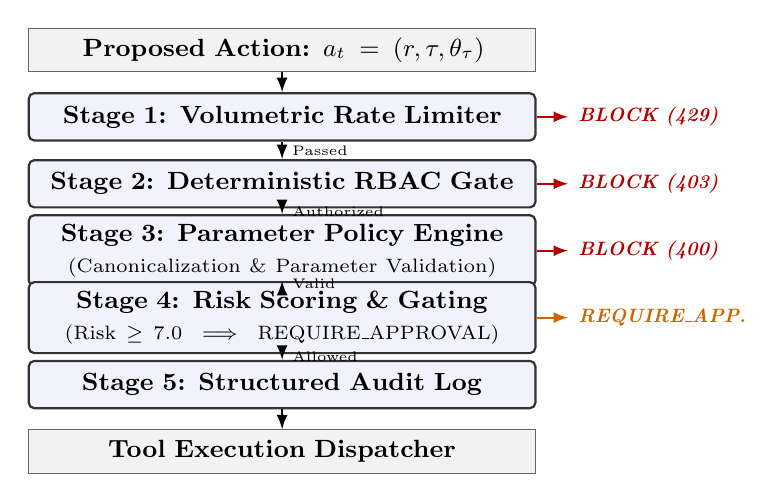
\begin{tikzpicture}[
    node distance=0.85cm,
    stage/.style={rectangle, draw=black!80, fill=blue!5, thick, text width=6.2cm, align=center, rounded corners=2pt, minimum height=0.6cm, font=\small},
    io/.style={rectangle, draw=black!60, fill=gray!10, text width=6.2cm, align=center, minimum height=0.55cm, font=\small},
    action/.style={font=\scriptsize\itshape, text=red!70!black},
    arrow/.style={-latex, thick}
]
    \node[io] (input) {\textbf{Proposed Action:} $a_t = (r, \tau, \theta_\tau)$};
    \node[stage, below of=input] (s1) {\textbf{Stage 1: Volumetric Rate Limiter}};
    \node[stage, below of=s1] (s2) {\textbf{Stage 2: Deterministic RBAC Gate}};
    \node[stage, below of=s2] (s3) {\textbf{Stage 3: Parameter Policy Engine}\\\scriptsize(Canonicalization \& Parameter Validation)};
    \node[stage, below of=s3] (s4) {\textbf{Stage 4: Risk Scoring \& Gating}\\\scriptsize($\text{Risk} \ge 7.0 \implies \text{REQUIRE\_APPROVAL}$)};
    \node[stage, below of=s4] (s5) {\textbf{Stage 5: Structured Audit Log}};
    \node[io, below of=s5] (exec) {\textbf{Tool Execution Dispatcher}};

    \draw[arrow] (input) -- (s1);
    \draw[arrow] (s1) -- node[right, font=\tiny] {Passed} (s2);
    \draw[arrow] (s2) -- node[right, font=\tiny] {Authorized} (s3);
    \draw[arrow] (s3) -- node[right, font=\tiny] {Valid} (s4);
    \draw[arrow] (s4) -- node[right, font=\tiny] {Allowed} (s5);
    \draw[arrow] (s5) -- (exec);

    \draw[arrow, red!70!black] (s1.east) -- ++(0.4,0) node[right, action] {\textbf{BLOCK (429)}};
    \draw[arrow, red!70!black] (s2.east) -- ++(0.4,0) node[right, action] {\textbf{BLOCK (403)}};
    \draw[arrow, red!70!black] (s3.east) -- ++(0.4,0) node[right, action] {\textbf{BLOCK (400)}};
    \draw[arrow, orange!80!black] (s4.east) -- ++(0.4,0) node[right, font=\scriptsize\itshape, text=orange!80!black] {\textbf{REQUIRE\_APP.}};
\end{tikzpicture}
\caption{Sequential multi-stage tool governance pipeline in \textbf{PromptAegis}.}
\label{fig:pipeline}
\end{figure}

\subsection{Complete Mediation Scope}
PromptAegis provides application-level complete mediation strictly for structured tool invocations explicitly dispatched to its interface. Crucially, this operational boundary entails three explicit security constraints:
\begin{enumerate}
    \item \textbf{Routed Tool Calls}: Every structured tool invocation dispatched to the gateway interceptor is deterministically evaluated against rate limits, RBAC permissions, and parameter policies prior to execution dispatch.
    \item \textbf{Sub-Shell and Interpreter Boundary}: The gateway operates above the operating system syscall interface; if an agent is authorized to execute an unconstrained shell or code interpreter (e.g., \texttt{bash}, \texttt{python}), arbitrary commands executed internally within that sub-environment bypass parameter-level regex inspection.
    \item \textbf{Semantic Malice within Authorized Parameters}: Purely syntactic policy evaluation cannot detect semantically hostile actions that utilize valid syntax and authorized parameters (e.g., an authorized customer query retrieving unauthorized sensitive records).
\end{enumerate}

\section{Defensive Mechanisms}

\subsection{Stage 1: Volumetric Fixed Tumbling-Window Rate Limiter}
Implemented in \texttt{backend/governance/rate\_limiter.py}, Stage 1 partitions time into fixed 60-second intervals:
\begin{equation}
\text{BucketID}(t) = \left\lfloor \frac{t}{60.0} \right\rfloor
\end{equation}
For principal $p$ and tool $\tau$ with quota $L$, invocations are atomically counted in an SQLite store. Invocations where count exceeds $L$ within the current 60s bucket are rejected with HTTP 429.

\subsection{Stage 2: Deterministic RBAC Enforcement}
Stage 2 validates the role-to-tool permission relation $\mathcal{P} \subseteq \mathcal{R} \times \mathcal{T}$ via \texttt{backend/governance/permission\_engine.py}. If $(r, \tau) \notin \mathcal{P}$, execution is denied immediately without parameter processing.

\subsection{Stage 3: Parameter Canonicalization \& Policy Inspection}
Stage 3 in \texttt{backend/governance/policy\_engine.py} first canonicalizes string arguments:
\begin{itemize}
    \item \textbf{Keyword-Agnostic Base64 Decoding (\texttt{\_safe\_b64\_decode})}: Identifies Base64 candidates (\texttt{\^{}[A-Za-z0-9+/=]\{8,\}\$}). If decoding yields valid UTF-8 with $\ge 85\%$ printable ASCII characters, the parameter is unmasked in-place.
    \item \textbf{Bounded URL Percent-Unquoting}: Applies a bounded 2-pass \texttt{urllib.parse.unquote}.
    \item \textbf{SQL Comment Stripping}: Removes \texttt{-- ...\textbackslash n} and \texttt{/* ... */} fragments.
\end{itemize}
Canonicalized arguments are evaluated against compiled regular expressions bound to specific tool IDs.

\subsection{Stage 4: Risk Scoring \& Approval Gating}
Stage 4 computes a composite risk score based on tool severity, argument payloads, and historical frequency. If \texttt{requires\_approval} is enabled and the calculated score satisfies $\text{risk\_score} \ge 7.0$, the gateway issues \texttt{REQUIRE\_APPROVAL}, pausing dispatch.

\subsection{Stage 5: Structured Audit Logging}
Stage 5 persists structured audit records with execution timestamps, decision outcomes, latency measurements, and matched policy identifiers.

\section{Experimental Methodology \& Benchmark Construction}

\subsection{Primary Benchmark Composition}
The primary benchmark consists of $N=600$ scenarios:
\begin{itemize}
    \item \textbf{Synthetic Attack Corpus ($N=500$)}: 100 synthetic scenarios across each of the 5 primary threat categories (T1: Unauthorized Tool, T2: Privilege Escalation, T3: Restricted Execution, T4: Parameter Manipulation, T5: Excessive Calls), designed to systematically evaluate rule coverage against canonical injection patterns.
    \item \textbf{Benign Operational Corpus ($N=100$)}: 100 realistic operational commands reflecting standard software development and customer support tasks (e.g., \texttt{git status}, \texttt{search\_customer}, \texttt{read\_log\_file}). Scenario \texttt{LEG-098} tests parameter precision by updating an authorized customer record where a string argument legitimately includes \texttt{"password"}.
\end{itemize}

\subsection{Deterministic Research Clock}
To ensure bit-for-bit reproducibility, experiments run under \texttt{ResearchExperimentClock} (\texttt{experiments/research\_clock.py}). Virtual time advances deterministically by $\Delta t = 70.0\text{ s}$ under normalized evaluation (guaranteeing 0 rate-limiter events) and by $\Delta t = 0.05\text{ s}$ under burst stress evaluation.

\section{Mechanism-Isolation Ablation Study}
To prevent rate-limiter saturation from conflating semantic policy effectiveness, we evaluate six configurations across $3{,}000$ attack evaluations and $3{,}600$ total scenario decisions, reported in Table~\ref{tab:ablation}.

\begin{table*}[t]
\centering
\small
\caption{Benchmark results across 6 configurations ($3{,}000$ attack evaluations, $3{,}600$ total scenario decisions). Paired latency overhead reflects medians of paired per-scenario differences ($N=500$ pairs); unvalidated paired statistics for RBAC, Policy, and Hardened are omitted.}
\label{tab:ablation}
\begin{tabular}{lcccccccc}
\toprule
\textbf{Configuration} & \textbf{Arrival Regime ($\Delta t$)} & \textbf{Blocked ($N_{\text{block}}/500$)} & \textbf{ASR} & \textbf{LTCR} & \textbf{FPR} & \textbf{Median P50} & \textbf{Paired Overhead} \\
\midrule
\textbf{Baseline (Unprotected)} & Independent & $0 / 500$ & \textbf{100.0\%} & \textbf{100.0\%} ($100/100$) & \textbf{0.0\%} ($0/100$) & $7.35\text{ ms}$ & Reference ($0.00\text{ ms}$) \\
\textbf{RBAC Only} & Independent & $300 / 500$ & \textbf{40.0\%} & \textbf{100.0\%} ($100/100$) & \textbf{0.0\%} ($0/100$) & $8.09\text{ ms}$ & -- \\
\textbf{Policy Only} & Independent & $335 / 500$ & \textbf{33.0\%} & \textbf{100.0\%} ($100/100$) & \textbf{0.0\%} ($0/100$) & $8.99\text{ ms}$ & -- \\
\textbf{Full Normalized} & $\Delta t = 70.0\text{ s}$ & $350 / 500$ & \textbf{30.0\%} & \textbf{100.0\%} ($100/100$) & \textbf{0.0\%} ($0/100$) & $19.08\text{ ms}$ & \textbf{+11.27 ms} \\
\textbf{Full Burst} & $\Delta t = 0.05\text{ s}$ & $370 / 500$ & \textbf{26.0\%} & \textbf{100.0\%} ($100/100$) & \textbf{0.0\%} ($0/100$) & $20.43\text{ ms}$ & \textbf{+13.38 ms} \\
\textbf{Hardened Governance} & $\Delta t = 0.05\text{ s}$ & $366 / 500$ & \textbf{26.8\%} & \textbf{100.0\%} ($100/100$) & \textbf{0.0\%} ($0/100$) & $24.21\text{ ms}$ & -- \\
\bottomrule
\end{tabular}
\end{table*}

\subsection{Key Findings}
\begin{enumerate}
    \item \textbf{Isolated Semantic Performance}: Under \texttt{Full Normalized}, exactly \textbf{0 rate-limiting blocks occur}. Semantic controls alone achieve a \textbf{$30.0\%$ ASR} ($350/500$ blocked). RBAC neutralizes Categories T1--T3 ($300$ blocks), while Policy catches 50 parameter injections (T4).
    \item \textbf{Compound Burst Regime}: Under \texttt{Full Burst}, high-frequency traffic trips the rate limiter, reducing ASR to $26.0\%$. This reduction is a compound operational effect resulting from traffic density, not a semantic gain.
\end{enumerate}

\section{Calibrated Gateway Evaluation}
We evaluate a calibrated gateway configuration featuring refined argument schemas and tool-scoped parameter fallback rules. The calibrated parameter rules (SQL injection regex on \texttt{query} arguments; restricted field guard scoped to \texttt{update\_customer}) were designed and evaluated on the same $N=600$ canonical benchmark corpus; no held-out evaluation split was employed.
\begin{itemize}
    \item \textbf{Calibrated Attack Success Rate (ASR)}: \textbf{$20.4\%$} ($102/500$ allowed, $398/500$ blocked; the full gateway stack, including rate limiting, is active in this configuration).
    \item \textbf{Utility Preservation}: \textbf{$100.0\%$ LTCR} ($100/100$ completed), \textbf{$0.0\%$ FPR} ($0/100$ blocked).
    \item \textbf{Resolution of \texttt{LEG-098}}: Scoping parameter rules strictly to \texttt{update\_customer} prevents false rejections of legitimate strings containing \texttt{"password"}.
    \item \textbf{Latency Profile}: Median calibrated processing time is \textbf{$23.73\text{ ms}$} (P50).
\end{itemize}

\section{Adversarial Robustness Evaluation}
We evaluate 500 adversarial mutation instances structured as 5 perturbation transformation classes applied to 100 shared base attack templates ($5 \times 100 = 500$ instances). This clustered design evaluates evasion robustness across transformation types rather than 500 independent samples. Each instance is evaluated under Standard and Hardened configurations across two operational regimes, yielding $2{,}000$ execution-level evaluations in total.

\subsection{Regime A: Mechanism-Isolated Policy Evaluation (Rate Limiter Inactive)}
Isolates pure regex and canonicalization recall across $1{,}000$ execution evaluations, reported in Table~\ref{tab:regime_a}.

\begin{table}[h]
\centering
\scriptsize
\caption{Regime A adversarial results isolating semantic parameter inspection ($1{,}000$ execution evaluations).}
\label{tab:regime_a}
\begin{tabular}{lccccc}
\toprule
\textbf{Mutation Class} & \textbf{Instances} & \textbf{Standard Block} & \textbf{Hardened Block} & \textbf{Delta} & \textbf{Standard ASR} \\
\midrule
\texttt{case\_alt.} & 100 & $50.0\%$ ($50/100$) & $33.0\%$ ($33/100$) & $-17.0\%$ & $50.0\%$ \\
\texttt{comment\_frag.} & 100 & $50.0\%$ ($50/100$) & $33.0\%$ ($33/100$) & $-17.0\%$ & $50.0\%$ \\
\texttt{advanced\_sql} & 100 & $50.0\%$ ($50/100$) & $33.0\%$ ($33/100$) & $-17.0\%$ & $50.0\%$ \\
\texttt{url\_encoding} & 100 & $50.0\%$ ($50/100$) & $33.0\%$ ($33/100$) & $-17.0\%$ & $50.0\%$ \\
\textbf{\texttt{base64\_obf.}} & 100 & \textbf{0.0\%} ($0/100$) & \textbf{50.0\%} ($50/100$) & \textbf{+50.0\%} & \textbf{100.0\%} \\
\midrule
\textbf{Overall} & \textbf{500} & \textbf{40.0\%} ($200/500$) & \textbf{36.4\%} ($182/500$) & \textbf{-3.6\%} & \textbf{60.0\%} \\
\bottomrule
\end{tabular}
\end{table}

\subsection{Regime B: Compound Burst Gateway Evaluation ($\Delta t = 0.05\text{ s}$)}
Evaluates the full runtime gateway under rapid arrival across $1{,}000$ execution evaluations, reported in Table~\ref{tab:regime_b}.

\begin{table}[h]
\centering
\scriptsize
\caption{Regime B compound burst results ($1{,}000$ execution evaluations). Attack Success Rates are 24.8\% (Standard) and 25.6\% (Hardened).}
\label{tab:regime_b}
\begin{tabular}{lcccc}
\toprule
\textbf{Mutation Class} & \textbf{Std Burst Block} & \textbf{Hard Burst Block} & \textbf{Delta} & \textbf{Attribution (Std)} \\
\midrule
\texttt{case\_alt.} & $76.0\%$ ($76/100$) & $74.0\%$ ($74/100$) & $-2.0\%$ & Policy: 4, RateLim: 72 \\
\texttt{comment\_frag.} & $76.0\%$ ($76/100$) & $74.0\%$ ($74/100$) & $-2.0\%$ & Policy: 4, RateLim: 72 \\
\texttt{advanced\_sql} & $76.0\%$ ($76/100$) & $74.0\%$ ($74/100$) & $-2.0\%$ & Policy: 4, RateLim: 72 \\
\texttt{url\_encoding} & $76.0\%$ ($76/100$) & $74.0\%$ ($74/100$) & $-2.0\%$ & Policy: 4, RateLim: 72 \\
\texttt{base64\_obf.} & $72.0\%$ ($72/100$) & $76.0\%$ ($76/100$) & $+4.0\%$ & Policy: 0, RateLim: 72 \\
\midrule
\textbf{Overall} & \textbf{75.2\%} ($376/500$) & \textbf{74.4\%} ($372/500$) & \textbf{-0.8\%} & \textbf{RateLim: 360, Pol: 16} \\
\bottomrule
\end{tabular}
\end{table}

\subsection{Attribution and Non-Monotonicity Findings}
\begin{itemize}
    \item \textbf{Base64 Canonicalization Gain}: Standard regex exhibits $0.0\%$ detection on Base64 payloads; keyword-agnostic canonicalization increases block rate to $50.0\%$ ($50/100$).
    \item \textbf{Non-Monotonic Rule Trade-off}: Stripping comments alters string character offsets, degrading secondary regex trigger rates in multi-stage payloads ($50\% \to 33\%$). Overall isolated block rate decreases from $40.0\%$ to $36.4\%$.
    \item \textbf{Rate-Limiter Dominance in Burst}: In Regime B, \textbf{$95.74\%$ ($360/376$)} of blocked attacks in the standard pipeline are enforced by the rate limiter. Burst results reflect volumetric throttling rather than semantic normalization.
\end{itemize}

\section{Rate-Limit Stress Evaluation}
Evaluating the fixed 60-second tumbling window across quotas $L \in \{5, 20, 100\}$ confirms exact saturation:
\begin{itemize}
    \item Limit 5: Requests 1--5 allowed; Request \#6 blocked ($429\text{ Too Many Requests}$) at $t=5.0\text{s}$.
    \item Limit 20: Request \#21 blocked at $t=20.0\text{s}$.
    \item Limit 100: Request \#101 blocked at $t=100.0\text{s}$.
    \item Reset: Advancing virtual time across the tumbling boundary to $t=61.0\text{s}$ resets the counter, allowing Request \#7.
\end{itemize}

\section{Exploratory Closed-Loop LLM Agent Pilot}
An exploratory evaluation ($N=20$) integrated PromptAegis into a multi-turn ReAct agent powered by \texttt{openai/gpt-oss-120b}:
\begin{itemize}
    \item \textbf{Compromise Induction Rate}: The LLM succumbed to prompt injection in \textbf{$40.0\%$} ($4/10$) of attack episodes, generating unauthorized tool invocations.
    \item \textbf{Conditional Interception Rate}: PromptAegis intercepted \textbf{$75.0\%$} ($3/4$) of these compromised tool calls post-generation.
    \item \textbf{End-to-End System Breach Rate}: Only \textbf{$10.0\%$} ($1/10$) of attacks resulted in unintercepted tool execution in the target environment.
    \item \textbf{Benign Completion (LTCR)}: \textbf{$100.0\%$} ($10/10$) of benign tasks completed.
    \item \textbf{Latency Accounting}: Mean model inference latency was $755.83\text{ ms}$; mean gateway inspection latency was $161.11\text{ ms}$ (prompt-level ratio \textbf{$21.32\%$}). During active tool governance cycles, gateway overhead was $230.16\text{ ms}$ against $723.74\text{ ms}$ execution (tool-level ratio \textbf{$31.80\%$}).
    \item \textbf{Scope Note}: This pilot demonstrates operational feasibility in a live loop but is underpowered for general multi-model statistical claims.
\end{itemize}

\section{Statistical Analysis}
\begin{itemize}
    \item \textbf{McNemar Tests}: Pairwise Edwards continuity-corrected $\chi^2$ tests against the baseline ($N=500$ pairs):
    \begin{itemize}
        \item Normalized vs Baseline: $\chi^2 = 348.0029, p = 1.15 \times 10^{-77}$
        \item RBAC vs Baseline: $\chi^2 = 298.0033, p = 8.97 \times 10^{-67}$
        \item Policy vs Baseline: $\chi^2 = 333.0030, p = 2.13 \times 10^{-74}$
    \end{itemize}
    Each tested treatment differed significantly from the unprotected baseline under the paired McNemar analysis ($p < 10^{-66}$).
    \item \textbf{Paired Latency Tests}: Wilcoxon signed-rank tests reject the null hypothesis of zero latency overhead ($p < 10^{-80}$). Documented paired overheads ($+11.27\text{ ms}$ normalized, $+13.38\text{ ms}$ burst) reflect medians of paired per-scenario differences ($d_i = L_{\text{treatment}, i} - L_{\text{baseline}, i}$).
    \item \textbf{Bootstrap Confidence Intervals}: 10,000 bootstrap resamples yielded 95\% confidence intervals: Full Normalized ASR $[26.0\%, 34.0\%]$; RBAC ASR $[35.8\%, 44.2\%]$; Policy ASR $[29.0\%, 37.2\%]$.
\end{itemize}

\section{Security--Utility--Latency Trade-offs}
Evaluating security, utility, and execution latency concurrently:
\begin{itemize}
    \item \textbf{Security Reduction}: Attack success rate decreases from $100.0\%$ to $30.0\%$ under normalized semantic governance and to $20.4\%$ under calibrated configuration.
    \item \textbf{Utility Preservation}: All configurations achieved $100.0\%$ LTCR and $0.0\%$ FPR on the benign benchmark.
    \item \textbf{Measured Latency Cost}: The median paired overhead is $+11.27\text{ ms}$ under normalized traffic; in the closed-loop pilot, gateway inspection averaged $161.11\text{ ms}$ relative to $755.83\text{ ms}$ for model generation, corresponding to a $21.32\%$ prompt-level overhead ratio.
\end{itemize}

\section{Failure Modes and Negative Findings}
\begin{enumerate}
    \item \textbf{Semantic Parameter Smuggling}: In the closed-loop pilot, an injection induced the agent to call an authorized tool (\texttt{search\_customer}) with valid syntax (\texttt{query: "all\_customer\_emails"}). Because the command was syntactically benign and permitted under the active role, the gateway allowed it. Purely syntactic reference monitors cannot infer semantic intent.
    \item \textbf{Non-Monotonic Normalization}: Stripping comments altered string offsets, degrading secondary regex triggers and reducing isolated block rate from $40.0\%$ to $36.4\%$.
    \item \textbf{Burst Rate-Limiter Attribution}: $95.74\%$ of burst blocks are caused by rate limiting, not semantic inspection.
    \item \textbf{Encoding Depth Limitations}: Single-pass Base64 decoding unmasked $50.0\%$ of payloads, but multi-nested or custom encodings evaded detection.
\end{enumerate}

\section{Threats to Validity}
\begin{itemize}
    \item \textbf{Internal Validity}: Benchmark results depend on synthetic attack templates.
    \item \textbf{External Validity}: Closed-loop testing evaluated a single model (\texttt{gpt-oss-120b}). Generalization across diverse model families remains unmeasured.
    \item \textbf{Gateway Bypass Scope}: Direct OS execution within an unconstrained shell bypasses parameter-level inspection.
    \item \textbf{Tumbling-Window Boundary Effect}: Fixed tumbling windows permit boundary clustering ($2L$ calls within 2 seconds across the 60s reset).
\end{itemize}

\section{Related Work}
A comparative architectural taxonomy is presented in Table~\ref{tab:related_work}.

\begin{table*}[t]
\centering
\small
\caption{Architectural comparison of LLM safety and execution governance approaches.}
\label{tab:related_work}
\begin{tabular}{lllll}
\toprule
\textbf{Framework / Paradigm} & \textbf{Enforcement Point} & \textbf{Primary Mechanism} & \textbf{Determinism} & \textbf{Tool Mediation Scope} \\
\midrule
\textbf{System Prompt Instructions}~\cite{perez} & Prompt Input & Natural language instructions & Probabilistic & Unmediated \\
\textbf{RLHF Alignment}~\cite{ouyang} & Model Weights & Preference fine-tuning & Probabilistic & Unmediated \\
\textbf{Llama Guard}~\cite{llamaguard} & Token Stream & Secondary 7B LLM classifier & Probabilistic & Prompt/response safety classification \\
\textbf{NeMo Guardrails}~\cite{nemoguardrails} & Input/Output Dialog & Colang programmable dialog flows & Hybrid & Programmable action gating \\
\textbf{Guardrails AI}~\cite{guardrails} & Output Parser & RAIL specifications \& validator pipelines & Rule / validator-dependent & Input/output validation \& structural constraints \\
\textbf{OS Sandboxes (Docker/Seccomp)}~\cite{merkel,kerrisk_book} & Kernel Syscall & Cgroups~\cite{kerrisk_book,kerrisk_cgroups}, namespaces~\cite{kerrisk_book,kerrisk_namespaces}, seccomp~\cite{kerrisk_seccomp} & Deterministic & Process isolation \& selective syscall filtering \\
\textbf{PromptAegis (Ours)} & \textbf{Tool Dispatch Interface} & \textbf{RBAC, Normalization, Policy, Rate Limit} & \textbf{Deterministic} & \textbf{Complete routed tool-call mediation} \\
\bottomrule
\end{tabular}
\end{table*}

Prior research in agent security largely emphasizes input filtering~\cite{perez,llamaguard} or conversational flow management~\cite{nemoguardrails}. While Llama Guard~\cite{llamaguard} inspects conversational tokens, secondary classifiers introduce additional model inference passes. NeMo Guardrails~\cite{nemoguardrails} provides programmable dialogue and execution-flow constraints, whereas PromptAegis evaluates concrete structured tool calls using explicit RBAC matrices, parameter canonicalization, and rate limits. PromptAegis adapts classical reference monitor principles~\cite{anderson,schneider} to the structured tool-dispatch path.

\section{Limitations}
\begin{itemize}
    \item \textbf{Syntactic Bound}: PromptAegis inspects structured parameters via schemas and regexes; it does not perform semantic reasoning.
    \item \textbf{Enforcement Path Dependence}: The gateway protects only tools routed through its interface.
    \item \textbf{Exploratory Pilot Scale}: The closed-loop pilot ($N=20$) is an initial proof-of-concept.
    \item \textbf{In-Sample Calibration}: The calibrated gateway configuration was evaluated on the same benchmark corpus used to design the parameter rules; out-of-sample generalization of the calibrated configuration has not been established.
\end{itemize}

\section{Conclusion}
Securing autonomous LLM agents requires decoupling cognitive reasoning from concrete downstream execution. The PromptAegis gateway demonstrates that an application-level, deterministic reference monitor can reduce attack success rates from $100.0\%$ to $30.0\%$ under normalized semantic governance and to $20.4\%$ under calibrated configuration on the evaluated benchmark, while preserving $100.0\%$ benign task completion with a median paired overhead of $+11.27\text{ ms}$. However, protection remains bounded by policy expressiveness, cannot prevent semantic parameter smuggling within authorized domains, and does not alter the underlying vulnerability of the reasoning model.

\section{Reproducibility \& Artifact Availability}
All evaluation datasets, configuration files, and execution scripts are frozen:
\begin{itemize}
    \item \textbf{Repository}: \url{https://github.com/Shriram28Baskar/PromptAegis_RI}
    \item \textbf{Frozen Baseline Commit}: \texttt{f16fae2cffece5b032e47bb7dfc52220c2eae1fc}
    \item \textbf{Verification}: \texttt{python -m pytest tests/test_provenance_and_reproducibility.py} passes 5/5 assertions. Complete reproduction executes via \texttt{python experiments/run_all.py}.
\end{itemize}

\begin{thebibliography}{18}

\bibitem{react}
S.~Yao, J.~Zhao, D.~Yu, N.~Du, I.~Shafran, K.~Narasimhan, and Y.~Cao, ``ReAct: Synergizing Reasoning and Acting in Language Models,'' in \emph{Proc. Int. Conf. Learn. Represent. (ICLR)}, 2023.

\bibitem{toolformer}
T.~Schick, J.~Dwivedi-Yu, R.~Dess\`i, R.~Raileanu, M.~Lomeli, L.~Zettlemoyer, N.~Cancedda, and T.~Scialom, ``Toolformer: Language Models Can Teach Themselves to Use Tools,'' in \emph{Proc. Conf. Neural Inf. Process. Syst. (NeurIPS)}, 2023.

\bibitem{autogen}
Q.~Wu, G.~Bansal, J.~Zhang, Y.~Wu, B.~Li, E.~Zhu, L.~Jiang, X.~Zhang, S.~Zhang, J.~Liu, A.~H. Awadallah, R.~W. White, D.~Burger, and C.~Wang, ``AutoGen: Enabling Next-Gen LLM Applications via Multi-Agent Conversation,'' \emph{arXiv preprint arXiv:2308.08155}, 2023.

\bibitem{saltzer}
J.~H. Saltzer and M.~D. Schroeder, ``The Protection of Information in Computer Systems,'' \emph{Proc. IEEE}, vol.~63, no.~9, pp.~1278--1308, 1975.

\bibitem{merkel}
D.~Merkel, ``Docker: Lightweight Linux Containers for Consistent Development and Deployment,'' \emph{Linux Journal}, vol.~2014, no.~239, 2014.

\bibitem{greshake}
K.~Greshake, S.~Abdelnabi, S.~Mishra, C.~Endres, T.~Holz, and M.~Fritz, ``Not what you've signed up for: Compromising Real-World LLM-Integrated Applications with Indirect Prompt Injection,'' in \emph{Proc. ACM Workshop Offensive Technol. (WOOT)}, 2023.

\bibitem{ouyang}
L.~Ouyang, J.~Wu, X.~Jiang, D.~Almeida, C.~L. Wainwright, P.~Mishkin, C.~Zhang, S.~Agarwal, K.~Slama, A.~Ray, et~al., ``Training language models to follow instructions with human feedback,'' in \emph{Proc. Conf. Neural Inf. Process. Syst. (NeurIPS)}, 2022.

\bibitem{perez}
F.~Perez and I.~Ribeiro, ``Ignore Previous Prompt: Attack Techniques For Language Models,'' in \emph{Proc. NeurIPS Workshop on ML Safety}, 2022 (arXiv:2211.09527).

\bibitem{llamaguard}
H.~Inan, K.~Upasani, J.~Chi, R.~Rungta, K.~Iyer, Y.~Mao, M.~Tontchev, Q.~Hu, B.~Fuller, D.~Testuggine, and M.~Khabsa, ``Llama Guard: LLM-based Input-Output Safeguard for Human-AI Conversations,'' \emph{arXiv preprint arXiv:2312.06674}, 2023.

\bibitem{nemoguardrails}
T.~Rebedea, R.~Dinu, M.~Sreedhar, C.~Parisien, and J.~Cohen, ``NeMo Guardrails: A Toolkit for Controllable and Safe LLM Applications,'' \emph{arXiv preprint arXiv:2310.10501}, 2023.

\bibitem{zou}
A.~Zou, Z.~Wang, J.~Z. Kolter, and M.~Fredrikson, ``Universal and Transferable Adversarial Attacks on Aligned Language Models,'' \emph{arXiv preprint arXiv:2307.15043}, 2023.

\bibitem{anderson}
J.~P. Anderson, ``Computer Security Technology Planning Study,'' Tech. Rep. ESD-TR-73-51, Air Force Electronic Systems Division, 1972.

\bibitem{schneider}
F.~B. Schneider, ``Enforceable Security Policies,'' \emph{ACM Trans. Inf. Syst. Secur.}, vol.~3, no.~1, pp.~30--50, 2000.

\bibitem{guardrails}
Guardrails AI, ``Guardrails: Adding Guardrails to Large Language Models,'' \emph{GitHub Repository}, \url{https://github.com/guardrails-ai/guardrails}, 2023.

\bibitem{kerrisk_book}
M.~Kerrisk, \emph{The Linux Programming Interface: A Linux and UNIX System Programming Handbook}, No Starch Press, San Francisco, CA, 2010.

\bibitem{kerrisk_namespaces}
M.~Kerrisk, ``namespaces(7) --- overview of Linux namespaces,'' in \emph{Linux Programmer's Manual}, Linux Man-Pages Project, 2023.

\bibitem{kerrisk_cgroups}
M.~Kerrisk, ``cgroups(7) --- Linux control groups,'' in \emph{Linux Programmer's Manual}, Linux Man-Pages Project, 2023.

\bibitem{kerrisk_seccomp}
M.~Kerrisk, ``seccomp(2) --- operate on Secure Computing state of the process,'' in \emph{Linux Programmer's Manual}, Linux Man-Pages Project, 2023.

\end{thebibliography}

\end{document}
